\documentclass[11pt,a4paper,twocolumn]{article}
\usepackage[utf8]{inputenc}
\usepackage[T1]{fontenc}
\usepackage{amsmath}
\usepackage{amssymb}
\usepackage{amsfonts}
\usepackage{graphicx}
\usepackage[spanish]{babel}
\usepackage{tcolorbox,booktabs,fourier,tabularx,wrapfig,multicol,caption, subcaption,tikz}
\usepackage{import} %Para poder añadir imagenes SVG
\usepackage[headings]{fancyhdr}
\usepackage[left=2cm,right=2cm,top=2cm,bottom=2cm]{geometry}

\graphicspath{{./imagenestermo/}}


\author{Franco Guardiani, Valentin Franzoi, Daiana Polo}
\title{
\includegraphics[width=.3\textwidth]{utn} \\ \textsc{Termodinámica} \\ \textsl{Resumen de fórmulas} \\ }
\date{2022}

%Comando título de cada unidad
\newcommand{\unidad}[2]{\begin{center}
		\fontsize{10}{10}\selectfont\color{gray!50!black}\scshape Unidad #1 \\
		\fontsize{14}{14}\selectfont \scshape #2
\end{center}}

\parindent=0pt 

\fancyfoot[C]{}
\fancyfoot[R]{\thepage}
\fancyhead[R]{\textsc{Termodinámica técnica}}
\renewcommand{\headrulewidth}{0pt}
\fancyfoot[L]{Franco Guardiani, Valentin Franzoi, Daiana Polo}

\begin{document}
	\pagestyle{fancy}
	\maketitle
	\section*{Nomenclatura}
	\begin{tabular}{r l}
		$m$ & Masa \\
		$M$ & Peso molecular \\
		$n$ & Número de moles \\
		$R$ & Constante del gas \\
		$\overline{R}$ & Constante universal de los gases \\
		$P$ & Presión \\
		$V$ & Volumen \\
		$Q$ & Calor \\
		$T$ & Temperatura \\
		$U$ & Energía interna \\
		$E_{c}$ & Energía cinética \\
		$E_{p}$ & Energía potencial \\
		$W$ & Trabajo \\
		$W_{c}$& Trabajo de circulación\\
		$c_{v}$ & Calor específico a volumen cte. \\
		$c_{p}$ & Calor específico a presión cte. \\
		$x_i$ & Fracción molar \\
		$g_i$ & Composición gravimétrica \\
		$h$ & Entalpía \\
		$s$ & Entropía \\
		$h_\textup{f}$ & Calor sensible \\
		$h_\textup{fg}$ & Calor latente \\
		
		
		
	\end{tabular}
	
	\newpage
	
	\section*{Conceptos}
		
	\textbf{Propiedades:} Características del sistema que depende de su estado, pero no de cómo se alcanza el estado.
	
	\textbf{Ley cero:} Establece que para un conjunto de sistema sometido a distintas temperaturas estos realizan intercambio de energía hasta alcanzar el equilibrio térmico.
	
	\textbf{Energía:} En mecánica se define como la capacidad para producir un trabajo, en termodinámica la definimos como la capacidad de producir cambios en los sistemas.
	
	\textbf{Entalpía:} Es una propiedad y representa la cantidad de energía que un sistema intercambia con su entorno.
%	definida como el flujo de energía térmica en los procesos químicos efectuados a presión constante cuando el único trabajo es de presión-volumen, es decir,
	
	\textbf{Sistema:} Porción finita de materia en el espacio elegida para el análisis.
	
	\textbf{Trabajo de circulación:} ($W_c$) Cantidad de energía que se entrega para mover una unidad de masa de un punto a otro.
	
	\textbf{Entalpía:} ``El flujo de energía térmica en los procesos químicos efectuados a presión constante cuando el único trabajo es de presión-volumen''-wiki
	\newpage
	
	
%	CONCEPTOS FUNDAMENTALES-------------------------------------------------------
%	BEGIN_FOLD

	\unidad{1}{Conceptos Fundamentales}
	
	\textbf{Sistemas:} haciendo referencia al intercambio de masa y energía se pueden clasificar en:
	\begin{center}
		\begin{tabular}{r | l} \vspace{.2cm}
			\textsl{Sistema cerrado} & no masa, sí energía\\ \vspace{.2cm}
			\textsl{Sistema abierto} & sí masa, sí energía\\ \vspace{.2cm}
			\textsl{Sistema aislado} & no masa, no energía\\ 
		\end{tabular}
	\end{center}
	
	El sistema abierto se subdivide en \emph{circulantes} y \emph{de régimen permanentes}.
	
	\textbf{Equilibrio termodinámico:} se debe cumplir:\\
	
		\begin{tabular}{r | l} \vspace{.2cm}
		\textsl{Equilibrio Químico} & composición cte \\ \vspace{.2cm}
		\textsl{Equilibrio Mecánico} & $\Delta P =0$ \\ \vspace{.2cm}
		\textsl{Equilibrio Térmico} & $\Delta T =0$
	\end{tabular}
	

\textbf{Procesos y Ciclos}

Cualquier transformación que experimenta un sistema se denomina \emph{proceso}.

Cualquier proceso cuyos estados finales e iniciales son idénticos se denomina \emph{ciclo}. Un ciclo puede ser \emph{reversible} (proceso cuasiestático) o \emph{no reversible}. \\

\textbf{Función puntual}
Conocida como \emph{ecuación de estado}, ubica un punto en la gráfica, no depende de la trayectoria. Es diferencial exacta ($d$). $(\textbf{P, V, T, h})$ \\

\textbf{Función trayectoria}
Se ubica mediante el área en la gráfica, depende de la trayectoria. Es diferencial inexacta ($\delta$). $(\textbf{Q, W, s})$ \\

\textbf{Energía}

``Capacidad que tiene la materia de producir trabajo en forma de movimiento, luz, calor, etc.'' Wiki\\

	\textbf{Calor y Trabajo}
	
	El \emph{calor} es una forma de energía que se transfiere entre dos sistemas y es debida a la diferencia de temperatura.
	
	El \emph{trabajo} es debido al movimiento de una parte de la frontera del sistema ante la acción de una fuerza.
	
	El calor y trabajo son las formas de \emph{energía en transición.}
	
	Convención de signos:
	
	\begin{center}
		\begin{tabular}{r | l}     \vspace{.2cm}
		$+W$ & Hecho por el sistema \\ \vspace{.2cm}
		$-W$ & Hecho sobre el sistema\\ \vspace{.2cm}
		$+Q$ & Sistema recibe calor \\ \vspace{.2cm}
		$-Q$ & Sistema entrega calor \\
	\end{tabular}
	\end{center}
%	END_FOLD
	
	
%	GASES IDEALES
%	BEGIN_FOLD
	\unidad{2}{Gases Ideales}

	\textbf{Energía interna:} es la energía térmica almacenada en un gas (tiene que ver con las vibraciones y los movimientos de las particulas). La Ley de Joule de la Energía interna establece que en un gas perfecto la misma es la función solo de la temperatura\\
	
	\textbf{\textsc{Primera ley de la Termodinámica}}\\

Por ley de la conservación de la energía "\textsl{el calor neto suministrado hacia (o por) el sistema es igual al trabajo neto realizado por (o hacia) el sistema en sus alrededores}".
	
%``En un sistema aislado no se crea ni se destruye energía, y solo pueden ocurrir transformaciones de una forma de energía a otra.'', mas modernamente se enuncia: ``El trabajo que un sistema cerrado intercambia con el medio en una transformación adiabática ($\mathcal{Q}=0$) depende del estado inicial del que parte y del estado final a que llega; con independencia de los estados intermedios por los que el sistema pasa.''
Para un sistema cerrado:
\begin{center}
	$\delta \mathcal{Q}=$ d$U +\delta \mathcal{W}$\\
	$\mathcal{Q}= \Delta U + \mathcal{W}$\\
\end{center}

	\textbf{Calor especifico} calor requerido para aumentar una unidad de masa una unidad de temperatura.\\
	
	\textbf{Calor latente}  es la cantidad de energía requerida por una sustancia para cambiar de fase.
	\begin{center}
		$\mathcal{Q}=m h_\textup{fg}$ 
	\end{center} 
	
	\textbf{Calor sensible} es la energía calorífica que suministrada a un cuerpo o un objeto, hace que aumente su temperatura sin afectar su estructura molecular y por lo tanto su fase.
	\begin{center}
		\begin{tabular}{r | l}
			\textsl{a presión cte } & $\mathcal{Q}=\Delta H= m c_{p}\Delta T$ \\ \vspace{.2cm}
			\textsl{a volumen cte } & $\mathcal{Q}=\Delta U = n c_{v}\Delta T$
		\end{tabular}
	\end{center}

	\textbf{Ecuación de Estado de Gases Ideales}
	
	Un gas ideal es aquel que no tiene \emph{fuerzas de atraccion intermolecular.}
	\begin{center}
		\textbf{$PV=mRT$}\\
		\textbf{$PV = n\overline{R}T$}
	\end{center}

	\textbf{Ley de Boyle-Mariote: } El volumen de una masa dada en un gas ideal varia inversamente con la presión absoluta cuando $T=cte$.
\begin{center}
	$V \alpha \dfrac{1}{P}$\\
\end{center}
	
	\textbf{Ley de Charles: } Si cualquier gas ideal se calienta a presión constante, su volumen cambia directamente con su temperatura absoluta. \begin{center}
		$V \alpha T$
	\end{center}
	\newpage

		\textsc{Mezcla de gases}\\
		
		
	\textbf{Ley de Dalton }
	
	La presión de una mezcla de gases es igual a la suma de las presiones parciales de los constituyentes; dicha presión es la que el gas ejercería si ocupara el volumen total de la mezcla a la misma temperatura.\begin{center}
		$P_{T}=P_{1}+P_{2}$
	\end{center}
	
	\textbf{Ley de Amagat }
	
	En una mezcla de gases el volumen total que la mezcla ocupa es igual a la suma de los volúmenes parciales correspondientes a cada componente. Donde el volumen parcial es el volumen que ocuparía cada componente sometido a la misma presión y temperatura de la mezcla. \begin{center}
		$V_{T}=V_{1}+V_{2}$
	\end{center}
%	END_FOLD
		

%-----------------------------------------------------------------------------------------
	\unidad{3}{Gases Reales}
	
	\textbf{Ecuación de Van der Waals}
	
	\textbf{Ecuación de Beattie-Brigdeman}
	
	\textbf{Coeficiente de comprensibilidad}
	
	\textsc{Mezcla de gases}\\
%	---------------------------------------------------------------------------------------------

%---------------------------------------------------------------------------------------------------
	
	\unidad{4}{Transformaciones}
	
	\textbf{Transformación Isocórica}
		
	\textbf{Transformación Isobárica}
	
	\textbf{Transformación Isotérmica}
	
	\textbf{Transformación Adiabática}
	
	\textbf{Transformación Politrópica}
%	-----------------------------------------------------------------------------------------------------------------

%---------------------------------------------------------------------------------------------------------
	
	\unidad{5}{Primer Principio}
	
	Primer principio aplicado a gases perfectos.\\
	
	\textbf{Sistemas abiertos}
	
	Falta...
	
	\begin{center}
		$Q=\Delta U + \Delta E_{c} + \Delta E_{p} + W_c + \Delta W$
	\end{center}
%	---------------------------------------------------------------------------------------------------------------
	
	
%	SEGUNDO PRINCIPIO-------------------------------------------------------------------------------------------------------
%	BEGIN_FOLD
	\unidad{6}{Segundo Principio}
	
	\textbf{Rendimiento:} la medida de éxito o eficiencia se determina como el cociente entre la energía útil (obtenida) y la energía absorbida (demandada).\begin{center}
		$\eta = \dfrac{\textsc{Energía Útil}}{\textsc{Energía Absorbida}}$
	\end{center}
%CAMBIE LA IMAGEN POR UNA EN FORMATO SVG PARA QUE NO CROPEE (si no les guste  pongan en modo comentario y descomenten la otra.)	
	\begin{figure}[ht]
		\centering
		\def\svgwidth{0.4\textwidth}
		\import{imagenestermo/}{maqsvg.pdf_tex}
	\end{figure}
	
%	\begin{figure}[h]
%	\centering
%	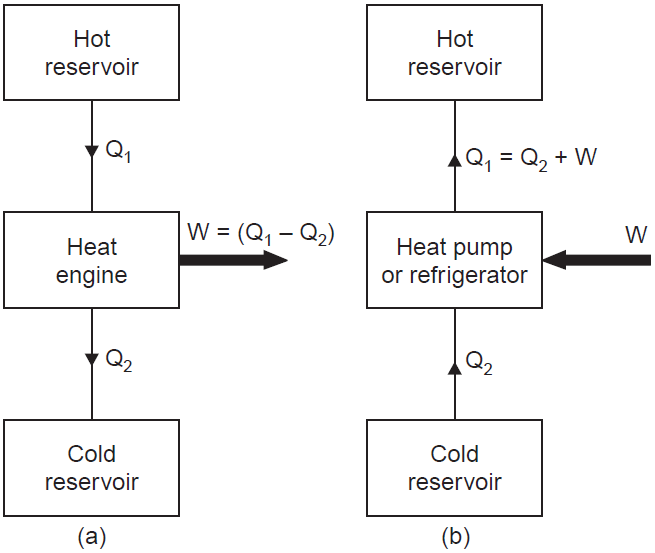
\includegraphics[width=.4\textwidth]{maquinas}
%	\end{figure}
%	
	\textbf{Máquina térmica:}
	Produce la máxima transferencia de trabajo a partir de una cantidad positiva de calor dada desde la fuente caliente. Transforma calor en trabajo mecanico operando \emph{cíclicamente}. (Fig. a)
	
	 La medida de éxito se denomina como eficiencia térmica:
	 \begin{center}
	 	$\eta_{mt}=\dfrac{W}{Q_{1}}=\dfrac{Q_{1}-Q_{2}}{Q_{1}} < 1$
	 \end{center}
	
	
	\textbf{Máquina térmica inversa:}
	\begin{itemize}
		\item \emph{Máquina frigorífica:} Produce la máxima transferencia de calor desde la fuente fría a partir de una transferencia de trabajo hacia la máquina. (Fig. b)
		\item \emph{Bomba de calor:} Produce la máxima transferencia de calor hacia la fuente caliente a partir de una transferencia de trabajo hacia la máquina.
	\end{itemize}
	
	 Los rendimientos o medidas de éxito para las máquinas térmicas inversas se denominan como \emph{coeficientes de desempeño}:
	 
	 \begin{center}
		COP$_{mf}=\dfrac{Q_{2}}{W}=\dfrac{Q_{2}}{Q_{1}-Q_{2}} > 1$ \\
		COP$_{bc}=\dfrac{Q_{1}}{W}=\dfrac{Q_{2}}{Q_{1}-Q_{2}} > 1$\\
	\end{center}

	
	
	\begin{center}
	\textsc{\textbf{Enunciado de Clausius}}
	
	\textsl{Considera la transformación de calor entre dos fuentes térmicas.} \\
	
	El calor, por sí mismo, no puede fluir de un cuerpo más frío a uno más caliente en un proceso cíclico. \vspace{.3cm}
	
	\textsc{\textbf{Enunciado de Kelvin-Planck}}
	
	\textsl{Considera la transformación de calor en trabajo}\\
	
	Es imposible obtener la extracción de calor de una sola fuente térmica y realizar la cantidad equivalente de trabajo sin producir ningún otro efecto.
	
	\end{center}
	
	\textbf{Temperatura termodinámica}
	
	En una fuente térmica \emph{la temperatura permanece uniforme y fija} ("$\infty$") y la transferencia de calor es función de dicha propiedad. Se puede expresar entonces:
	\begin{center}
		$\dfrac{Q_{1}}{Q_{2}}=\dfrac{T_{1}}{T_{2}}$
	\end{center}
	
	\textbf{Ciclo de Carnot}\\
	
		\begin{figure}[ht]
			\centering
			\def\svgwidth{0.3\textwidth}
			\import{imagenestermo/}{CicloCARNOT.pdf_tex}
		\end{figure}
	
	``El ciclo de Carnot es el más simple, debe ser reversible dado que la máquina térmica es reversible.''
%	``Todo ciclo reversible de una máquina térmica, que intercambia calor con dos fuentes, debe tener entre las transformaciones que lo integran una transformación isotérmica realizada a la temperatura de la fuente caliente.'' -García.\\
	
	\textit{Con nuestras palabras:} Carnot planteo un ciclo reversible (todas las transformaciones son reversibles), para que sea reversible el proceso de intercambio de calor, debe realizarse a través de un transformación isotérmica (porque el fluido debe tener la misma temperatura a la que la fuente lo cede/recibe, dado que una de transferencia de calor solo será reversible si el que cede/recibe calor y el que recibe/cede están a la misma temperatura). \\
	De lo anterior se concluye que todo ciclo reversible debe contar con 2 transformaciones (A-B y C-D):
	\begin{itemize}
		\item Una transformación isotérmica a la temperatura $T_{1}$, en la que el fluido intermediario recibe el calor $Q_{1}$ de la fuente caliente.
		\item Una transformación isotérmica a la temperatura $T_{2}$, en la que el fluido intermediario entrega el calor $Q_{2}$ a la fuente fría.
	\end{itemize}
	Estas dos transformaciones son imprescindibles, puesto que de lo contrario no habrá posibilidad de escribir un ciclo reversible.\\
	Para completar el ciclo Carnot utilizo dos transformaciones adiabáticas reversibles (B-C y D-A).\\
	Así se concibe el ciclo de Carnot, que estará constituido por dos isotérmicas y dos adiabáticas reversibles.\\
	El rendimiento del ciclo será:
	\begin{center}
		$\eta_{C}=1-\dfrac{Q_{2}}{Q_{1}}$\\
	\end{center}
Al ser reversible
	\begin{center}
		$\eta_{C}=1-\dfrac{T_{2}}{T_{1}}$\\
	\end{center}
	\newpage
	\underline{Etapas de un ciclo de Carnot de un cilindro (Rajput):}
	\begin{itemize}
		\item ETAPA 1: Proceso A-B, se aplica una fuente de energía caliente. El calor $Q_{1}$  se toma mientras el fluido se expande isotérmica y reversiblemente a una alta temperatura cte $T_{1}$.
		\item ETAPA 2: Proceso B-C, el cilindro se convierte en un aislante perfecto de manera que no tiene lugar un flujo térmico. El fluido se expande adiabática y reversiblemente mientras la temperatura disminuye de $T_{1}$ a $T_{2}$ 
		\item ETAPA 3: Proceso C-D, se aplica una fuente de energía fría. El calor $Q_{2}$ fluye del fluido mientras se comprime isotérmica y reversiblemente a una temperatura menor cte $T_{2}$.
		\item ETAPA 4: proceso D-A, la cabeza del cilindro se convierte en un aislante perfecto tal que no ocurre flujo de calor. La compresión continua adiabática y reversiblemente durante la cual la temperatura se aumenta de $T_{2}$ a $T_{1}$
	\end{itemize}
	
	
	
	
	\textbf{Teorema de Carnot}\\
	\textit{``Toda máquina térmica tendrá un rendimiento menor o igual que el de la máquina térmica reversible que funcione entre las mismas fuentes''} , para demostrarlo se recurre al absurdo (se plantea lo contrario).
	\begin{center}
		$\eta_{mt}\leq \eta_{mtR}$
	\end{center}
	Como derivado de ese teorema \textit{``Todas las máquinas reversibles que actúan entre dos fuentes a temperaturas constantes dadas tienen el mismo rendimiento, independiente de la naturaleza del sistema activo''}. En consecuencia el rendimiento de la máquina térmica reversivle sera independiente de 
	\begin{itemize}
		\item Del fluido intermediario empleado
		\item Del ciclo Termodinámico que describa el fluido
		\item De los dispositivos mecánicos que se utilizan en la máquina
	\end{itemize}

	Por lo que el rendimiento de la máquina será solo en funcion de las temperaturas de las fuentes entre las que funcione : $\eta_{R}=f(T_{1},T_{2})$
	\newpage
%	END_FOLD
	
%	ENTROPIA-------------------------------------------------------------------------
%	BEGIN_FOLD
	\unidad{7}{Entropía}
	\textbf{Desigualdad de Clausius}\\
	Se considera una máquina térmica que intercambia calor con tres fuentes a temperaturas $T_{1}> T_{2}> T_{0}$.\\
	La máquina recibe el calor de las fuentes calientes $T_{1},T_{2}$, cede el calor a la fuente fría $T_{0}$ y a otros cuerpos del medio un trabajo L.\\
	Es posible restablecer la situación en las fuentes introduciendo máquinas frigoríficas reversibles que quiten el calor de la fuente $T_{0}$ y entreguen a la fuente de $T_{x}$ una cantidad de calor igual en valor absoluto a $Q_{x}$, de esta forma se obtiene la instalación esquematizada:
	\begin{figure}[ht]
		\centering
		\def\svgwidth{0.3\textwidth}
		\import{imagenestermo/}{clausis1.pdf_tex}
	\end{figure}
	
	
	La instalación solo intercambia calor en definitiva con una sola fuente que es la que se encuentra a temperatura $T_{0}$, como una instalacion que solo intercambia calor con una sola fuente no puede ser una maq. térmica, \emph{(2° principio)} el trabajo resultante del funcionamiento no puede ser positivo, o es nulo o es negativo:
	\begin{center}
		$L+L_{F1}+L_{F2}\leq0 $
	\end{center}
	Y aplicando el primer principio de la Termodinámica y reemplazando:
	\begin{center}
		$L+L_{F1}+L_{F2}=Q_{0}+Q_{0F1}+Q_{0F2}$\\
		\vspace{0.1 cm}
		$Q_{0}+Q_{0F1}+Q_{0F2}\leq0$
	\end{center}
	La máquina térmica introduce modificaciones en el universo que pueden se eliminadas si el ciclo definido por la maq. térmica es reversible, las dos máq. frigoríficas reversibles restablecen la situación en la fuente de temperatura $T_{0}$ y consumen el trabajo que la máq. térmica había producido. (igualdad a cero) .\\
	En caso de que el ciclo definido por la maq. térmica sea irreversible, no pueden se eliminadas totalmente las modificaciones y la suma de calores da menor que cero, es decir, queda calor incorporado en la fuente $T_{0}$ que no puede ser retirado por las maq. frigorificas y a su vez que el trabajo neto sea consumido. Es decir, el funcionamiento es un consumo de trabajo y una entrega de calor que queda en $T_{0}$.\\
	Como las maq. frigoríficas son reversibles, el cociente entre los valores absolutos de las cantidades de calor que intercambia con las fuentes es igual al cociente entre las temperaturas absolutas:\\

	\begin{tabular}{r c l} \vspace{.2cm}
	$\dfrac{|Q_{F1}|}{Q_{0F1}}=\dfrac{T_{1}}{T_{0}} \rightarrow$&$Q_{0F1}=\dfrac{T_{0}}{T_{1}} |Q_{F1}|\rightarrow$	&$Q_{0F1}=\dfrac{T_{0}}{T_{1}} Q_{1}$ \\
	& &	$Q_{0F2}=\dfrac{T_{0}}{T_{2}} Q_{2}$\\	
	\end{tabular}
	Reemplazando y dividiendo todo por $T_{0}$:
	\begin{center}
		$Q_{0}+\frac{T_{0}}{T_{1}}Q_{1}+\frac{T_{0}}{T_{2}}Q_{2}\leq0$\\ 
		\vspace{0.2 cm}
		$\frac{Q_{0}}{T_{0}}+\frac{Q_{1}}{T_{1}}+\frac{Q_{2}}{T_{2}}\leq0$\\
		\vspace{0.2 cm}
		$\sum\frac{Q_{i}}{T_{i}}\leq0$\\
	\end{center}

	\textbf{Entropía}\\
	Es la posibilidad de que el calor se transforme en trabajo. Mayor entropia, menor posibilidad.
	\begin{center}
		$ds = \dfrac{\delta Q_{R}}{T}$\\
	\end{center}
    La entropía una funcion de estado.
    
    \begin{center}
    	Proceso reversible $\Delta S = 0$\\
    	Proceso irreversible $\Delta S < 0$\\
    \end{center}
	
	\textbf{\textsc{Primera ley de la Termodinámica}}\\
	``La entropía de todos los sólidos cristalinos perfectos es cero a temperatura absoluta cero
%	END_FOLD	
		
		
%	CALOR UTILIZABLE
%	BEGIN_FOLD
	\unidad{8}{Calor Utilizable}
	Analizamos el trabajo obtenido en una máquina térmica que opera entre dos fuentes de temperatura.
	dsdsa
		\begin{figure}[ht]
		\centering
		\def\svgwidth{0.2\textwidth}
		\import{imagenestermo/}{maqter.pdf_tex}
	\end{figure}
	
	Si consideramos que la máquina es reversible, sabemos que su rendimiento será máximo, por lo que el trabajo máximo obtenido por una máquina operando entre esas fuentes será:
	
	\begin{center}
		$L_{max}= \eta_{R} .Q_{1}$\\
		$L_{max}=(1-\frac{T_{0}}{T_{1}})Q_{1}$\\
	\end{center}
	A este máximo trabajo que podría obtenerse de la cantidad de calor lo llamaremos calor utilizable o Exergía:	
	\begin{center}
	$Q_{u}=Q_{1}-\dfrac{T_{0}}{T_{1}}$\\
	\end{center}
	Y al calor no utilizable lo llamaremos Anergía:
	\begin{center}
		$Q_{1}=Q_{u}+Q_{nu}$\\
	\end{center}
	La distribución de Exergía y Anergía de una cierta cantidad de calor depende de la temperatura de la fuente de la cual proviene.\\ %Si la temperatura T1 fuese infinita, todo el calor sería unicamente Exergía. En cambio si la fuente estuviera a igual temperatura que la atmosfera $T_{1}=T_{0}$ el calor que se suministre será totalmente Anergía.
	Para calcular el trabajo disponible en  una transformación de un sistema cerrado se debe calcular el trabajo total de la transformación y restarle el trabajo de dilatación el cual es:
	\begin{center}
	$L_{dil}=p_{0}(V_{0}-V_{1})$\\
	\end{center}

\textit{Lo que sigue es todo desarrollo, no se si se justifica copiar todo, resumir se complica.}\\
	\begin{tabular}{r | l} \vspace{.2cm}
		& \\ \vspace{.2cm}
		& \\ 
		
	\end{tabular}
	
	\unidad{9}{Funciones Características de Maxwell}
	\textit{No tengo idea que poner aca, muestra la relacion entre la entalpía, energía interna, etc. en funcion de S, T, V, p}\\	
	
	\begin{tabular}{r | l} \vspace{.2cm}
		& \\ \vspace{.2cm}
		& \\ 
		
	\end{tabular}
%	END_FOLD
	
%	VAPOR DE AGUA------------------------------------------------------------------
%BEGIN_FOLD
	\unidad{10}{Vapor de Agua}
	Regla de fase de Gibbs:
	\begin{center}
		$v=C+2-F$\\
	\end{center}	
%	\begin{itemize}
%		\item v= grado de libertad
%		\item C= Nro de sustancias
%		\item F= Nro de fases
%	\end{itemize}
	Definiciones:\\
	\textbf{Vapor saturado:} vapor que se encuentra en condiciones de equilibrio con su líquido.\\
	\textbf{Vapor sobrecalentado:} vapor que se encuentra a una temperatura superior a la de equilibrio con su líquido correspondiente a la presión a que está sometido.\\
	\textbf{Líquido saturado:} líquido que se encuentra en condiciones de equilibrio con su vapor.\\
	\textbf{Líquido comprimido:} líquido que está sometido a una presión mayor que la presión de equilibrio líquido-vapor correspondiente a la temperatura a que se encuentra.\\
	\textbf{Vapor húmedo:} mezcla de líquido y vapor saturados.\\
	
	Para poder analizar el valpor húmedo y los valores específicos de cualquier parámetro extensivo de la sustancia se necesita conocer el título/calidad del vapor:
	\begin{center}
		$\chi=\dfrac{m_{v}}{m_{v}+m_{L}}$\\
	\end{center}
	con este valor podemos calcular energía interna, entalpía, vol. especifico y entropía de nuestro vapor húmedo.	\\
	\textit{Lo que sigue en el Garcia de aca es como se forma un grafico de Mollier y uno Entropico, como que hace el desarrollo entre las Funciones caracteristicas y las regla de fases para encontrar las curvas de solido y de líquido.}
	
	
	
	
	\begin{tabular}{r | l} \vspace{.2cm}
		& \\ \vspace{.2cm}
		& \\ 
		
	\end{tabular}
	
	\unidad{11}{Máquinas de Vapor}
	
	
	\begin{tabular}{r | l} \vspace{.2cm}
		& \\ \vspace{.2cm}
		& \\ 
		
	\end{tabular}

	\unidad{12}{Ciclos Frigoríficos}

	
	\begin{tabular}{r | l} \vspace{.2cm}
		& \\ \vspace{.2cm}
		& \\ 
	\end{tabular}
%	END_FOLD
	
	%CICLOS DE MOTOR A GAS----------------------------------------------------------------
%	BEGIN_FOLD
	
	\unidad{13}{Ciclos de Motor a Gas}	
	\textbf{Ciclo}: es una serie repetida de procesos que ocurren en un cierto orden. Un ciclo ideal (máq. perfecta) no contempla perdidas por calor accidentales y sustancias de trabajo se suponen perfectas.\\
	\textbf{Eficiencia de aire estándar}: Para comparar diferentes ciclos es importante eliminar el efecto del poder calorífico del combustible, por ello se usa el aire como medio (supuesto como gas perfecto). Esto se conoce como eficiencia ideal.\\
	La eficiencia real de un ciclo es siempre menor que la eficiencia de aire estándar en condiciones ideales, se introduce un nuevo término ``Eficiencia relativa'', que es el cociente $\frac{Ef.~real}{Ef~aire~estandar}$\\
	\textbf{Suposiciones para el análisis}\\
	\begin{tabularx}{8cm}{X}
		$\bullet$ El gas de trabajo es un gas perfecto, sigue las leyes de gases ideales y tiene calores específicos constantes.\\
		$\bullet$ Las constantes físicas del gas son las mismas que las del aire a temperatura moderada.\\
		$\bullet$ Los procesos de compresión y expansión son adiabáticos y tienen lugar sin fricción interna (isentrópicos).\\
		$\bullet$ En el cilindro no ocurre reacción química. El calor se suministra o se rechaza poniendo en contacto con el cilindro una fuente caliente/fría en puntos apropiados.\\
		$\bullet$ El ciclo se considera cerrado con el mismo ``aire'' siempre.\\
	\end{tabularx}
	
	
	\textbf{Ciclo a volumen constante o ciclo Otto}\\
	
	\begin{center}
			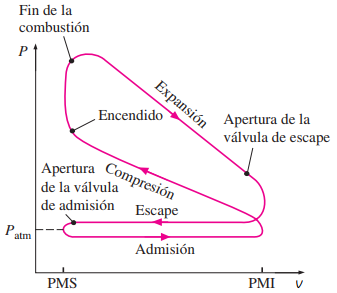
\includegraphics[width=5cm]{otto2}\\
	\end{center}

	Analizando desde el ciclo ideal, podemos hallar la eficiencia \textit{de aire estándar} o rendimiento térmico:

	\begin{center}
		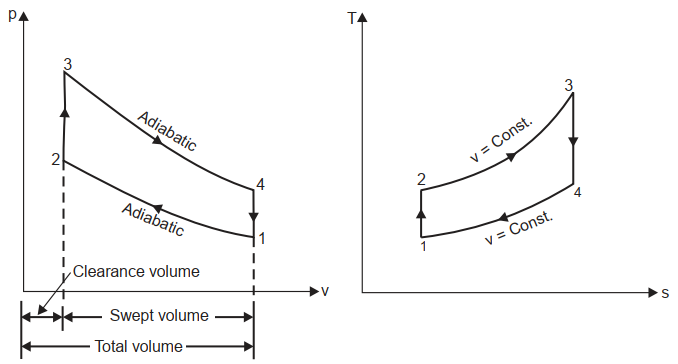
\includegraphics[width=7.5cm]{otto}
	\end{center}

	\begin{center}
		$\eta= \dfrac{c_{v}(T_{3}-T_{2})-c_{v}(T_{4}-T_{1})}{c_{v}(T_{3}-T_{2})}$\\ \vspace{0.2cm}
		$\eta=1-\dfrac{T_{4}-T_{1}}{T_{3}-T_{2}}$\\
	\end{center}

	Conociendo que la relación de compresión es igual a la relación de expansión, y que los puntos 1 y 2 , y los puntos 3 y 4 pertenecen a dos transformaciones adiabáticas, se cumple $T.v^{n-1}=cte$ para cada caso.\\
	
	\textit{La relación de compresión indica la relación entre el volumen del cilindro y la cámara de combustión.}
		\begin{tabular}{r l} 
			Relac. Compresión & $\frac{v_{1}}{v_{2}}$\\
			Relac. Expansión & $\frac{v_{4}}{v_{3}}$\\
		\end{tabular}
	
	Por ello $T_{2}$ y $T_{3}$ se pueden reescribir $T_{2}=T_{1}.r^{n-1}$ y $T_{3}=T_{4}.r^{n-1}$, reemplazando nos queda la eficiencia de aire estándar del ciclo Otto:

	\begin{center}
		$\eta=1-\dfrac{1}{r^{n-1}}$\\
	\end{center}
	Esta fórmula nos indica que a medida que aumenta la relación de compresión
	aumentará también el rendimiento, pero en la práctica la Rc no puede elevarse más
	allá de 9 o 10, ya que tanta compresión provocaría en la mezcla una preignición.\\	
	
	\textbf{Ciclo a presión constante o ciclo Diesel}\\
	Se diferencia del Otto en que permite obtener relaciones de compresión más elevadas,
	generalmente de 15 a 19, debido a que la inyección de combustible se realiza con
	posterioridad a la compresión del aire, que puede alcanzar presiones del orden de 40
	a 45 bar sin peligro de preignición. Ello trae como consecuencia un aumento del
	rendimiento térmico.
	\begin{center}
		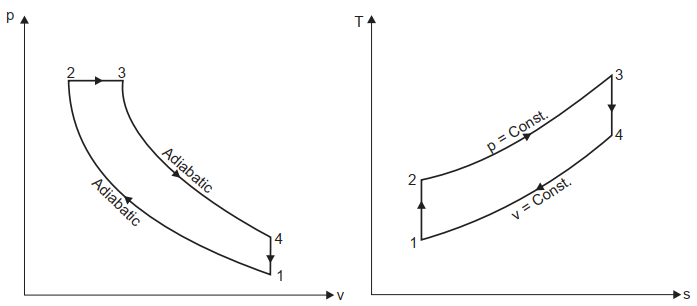
\includegraphics[width=8cm]{diesel}\\
		$\eta= \dfrac{c_{p}(T_{3}-T_{2})-c_{v}(T_{4}-T_{1})}{c_{p}(T_{3}-T_{2})}$\\
	\end{center}
	\begin{itemize}
		\item Coeficiente de la transformación $\gamma=\frac{c_{p}}{c_{v}}$
		\item Relación de compresión $r=\frac{v_{1}}{v_{2}}$  
		\item Relación de inyección $\phi=\frac{v_{3}}{v_{2}}$
	\end{itemize} 
	
	De cada transformación:
	
	\begin{itemize}
		\item De la 1-2 $\rightarrow T_{2}=T_{1}.r^{\gamma-1}$
		\item De la 2-3 $\rightarrow T_{3}=\phi .T_{2} = \phi T_{1}.r^{\gamma-1}$
		\item De la 3-4 $\rightarrow \frac{T_{3}}{T_{4}}=(\frac{v_{4}}{v_{3}})^{\gamma-1}=(\frac{r}{\phi})^{\gamma-1}\rightarrow T_{4}=T_{1}.\phi^{\gamma}$
	\end{itemize}
	
	Por lo que el rendimiento del ciclo Diesel es:
	\begin{center}
		\begin{tabular}{ r l }
		$ \eta =$&$ 1 -\dfrac{(T_{4}-T_{1})}{\gamma.(T_{3}-T_{2})}$\\[16pt]
		
		$ \eta =$&$1 -\dfrac{(T_{1}.\phi^{\gamma}-T_{1})}{\gamma.( \phi T_{1}.r^{\gamma-1}-T_{1}.r^{\gamma-1})}$\\[16pt]
		
		$ \eta =$&$1 -\dfrac{(\phi^{\gamma}-1)}{\gamma.r^{\gamma-1}.( \phi -1)}$\\[16pt]
		
		$ \eta =$&$1 - \dfrac{1}{\gamma.r^{\gamma-1}} . \dfrac{(\phi^{\gamma}-1)}{( \phi -1)}$\\	
	\end{tabular}
	\end{center}
		\textbf{Ciclo de combustión Dual o ciclo duplex}\\
	Combinación de los ciclos Otto y Diesel, de una manera en que el calor se agrega parcialmente a volumen y a presión constante, la ventaja del ciclo es que se dispone de más tiempo para suministrar combustible (se inyecta en el cilindro antes del final de la carrera de compresión) para la combustión. Debido a características de retardado de combustible este ciclo se utiliza invariablemente en motores Diesel y de encendido por zona caliente
	\begin{center}
		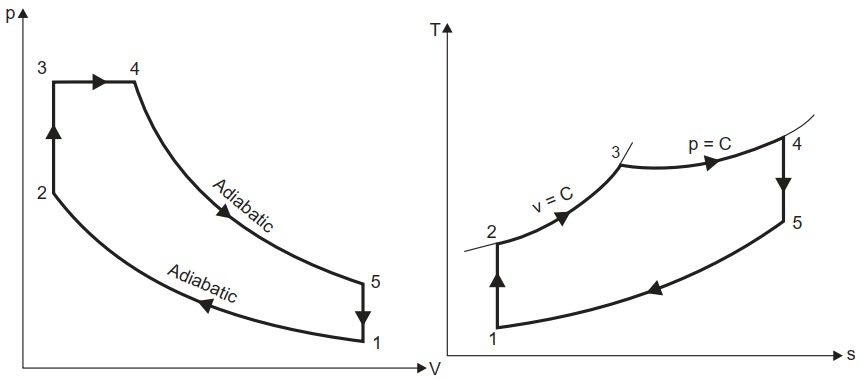
\includegraphics[width=8cm]{dual}
	\end{center}

	El rendimiento lo podemos escribir como:
	\begin{gather*}
		\eta =  \dfrac{Q_{2-3}+Q_{3-4}-Q_{5-1}}{Q_{2-3}+Q_{3-4}} = 1- \dfrac{Q_{5-1}}{Q_{2-3}+Q_{3-4}} \\
		\eta= 1- \dfrac{c_{v}(T_{5}-T_{1})}{c_{v}(T_{3}-T_{2})+c_{p}(T_{4}-T_{3})}\\
		\eta=1- \dfrac{(T_{5}-T_{1})}{(T_{3}-T_{2})+\gamma(T_{4}-T_{3})}
	\end{gather*}

	\textbf{Ciclo Brayton o Joule}\\
	Las transferencias de calor se dan a presión constante. Este ciclo describen las turbina de gas.
	\begin{center}
		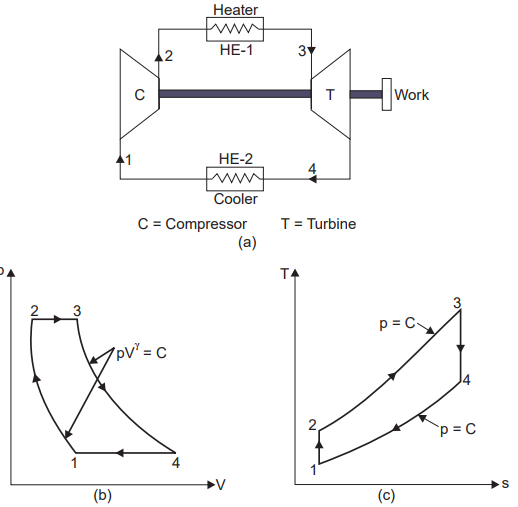
\includegraphics[width= .9\linewidth]{brayton1}
	\end{center}
	El rendimiento térmico del ciclo será:
	\begin{center}
		$\eta= \dfrac{c_{vp}(T_{3}-T_{2})-c_{p}(T_{4}-T_{1})}{c_{p}(T_{3}-T_{2})}$\\ \vspace{0.2cm}
		$\eta=1-\dfrac{T_{4}-T_{1}}{T_{3}-T_{2}}$\\
	\end{center}


Conociendo la relación de presión $r_{p}=\dfrac{p_{2}}{p_{1}}$
	\begin{itemize}
		\item De la 1-2 $\rightarrow T_{2}=T_{1}.r_{p}^{\frac{\gamma-1}{\gamma}}$
		\item De la 1-2 $\rightarrow T_{3}=T_{4}.r_{p}^{\frac{\gamma-1}{\gamma}}$
	\end{itemize}
Reemplazando quéda:
\begin{center}
	$	\eta = 1-\dfrac{1}{r_{p}^{\frac{\gamma-1}{\gamma}}}$\\
\end{center}
%	\begin{gather*}
%		\eta = 1-\dfrac{1}{r_{p}^{\frac{\gamma-1}{\gamma}}}\\
%%		\intertext{Donde la relación de presión $r_p$ es}
%%		r_{p} = \dfrac{p_2}{p_1}\\
%	\end{gather*}
	
	Vemos que el rendimiento aumenta a medida que aumenta la relación de presión, pero hasta un cierto límite:\\
	
	\begin{center}
		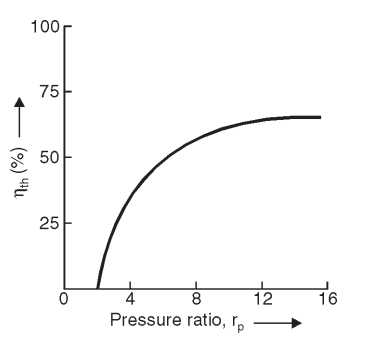
\includegraphics[width= .5\linewidth]{rendimientobrayton}
	\end{center}

	Por otra parte, fijada la temperatura de entrada de la turbina $T_3$, al crecer $r_p$, disminuirá el trabajo neto obtenido:
	
	\begin{gather*}
		W = W_{T} - W_{c} = c_{p}(T_{3} - T_{4}) - c_{p}(T_{3} - T_{4})\\
		\intertext{Desarrollando llegamos a}\\
		W = c_{p}T_{1}\left(\frac{T_{3}}{T_{1}} - r_{p}^{\frac{\gamma-1}{\gamma}}\right) \left(1- \dfrac{1}{r_{p}^{\frac{1-\gamma}{\gamma}}5} \right)
		\intertext{Para hallar el máximo trabajo neto derivamos respecto de $r_p$ y hallamos la máxima relación de presión}\\
		r_p = \left( \dfrac{T_{3}}{T_{1}} \right)^{\frac{\gamma}{2(\gamma - 1)}}
	\end{gather*}
	
	Los métodos para mejorar la eficiencia térmica de una planta de turbina de gas de ciclo abierto son:
	\begin{tabularx}{8cm}{X}
		$\bullet$ Enfriamiento intermedio\\
		$\bullet$ Recalentamiento\\
		$\bullet$ Regeneración\\
	\end{tabularx}
	%END_FOLD

	%COMPRESORES----------------------------------------------------------------------------
	%BEGIN_FOLD
		\unidad{14}{Compresores}
	Equipos cuya finalidad es suministrar gas a una presión mayor a aquella a que se dispone. El gas experimenta una transformación termodinámica abierta y nunca un ciclo.\\
	El compresor a embolo es un sistema abierto a flujo no permanente durante las carreras de admisión y escape, y un sistema cerrado durante la compresión, como todo el gas que penetra durante admisión es igual al gas que sale durante el escape se puede asimilar como un sistema circulante y operar con las expresiones del primer principio. $L_{c}=\int_{p_{1}}^{p_{2}} -v.dp$ , para una politrópica cualquiera queda:
	\begin{center}
			$L_{c} = \dfrac{m}{m-1} RT_{1} \left[  1- \left( \dfrac{p_{2}}{p_{1}}\right)  ^ {\frac{m-1}{m}} \right] $
	\end{center}
	\textbf{Espacio nocivo, rendimiento volumétrico}
	\begin{figure}[ht]
		\centering
		\def\svgwidth{0.3\textwidth}
		\import{imagenestermo/}{compresor.pdf_tex}
	\end{figure}

	La existencia de espacio nocivo reduce la capacidad de aspiración del compresor. Se denomina rendimiento volumétrico del compresor 
	\begin{center}
		$\eta_{v}=\frac{V_{a}}{V_{b}}$
	\end{center}
	El rendimiento dependerá de las presiones, el coeficiente de la politrópica, de la relación de espacio nocivo.
	\begin{center}
		$\epsilon_{0}=\frac{V_{o}}{V_{b}}$
	\end{center}
	Conociendo que $V_{a}=V_{b}-V_{1}$, trabajando:
	\begin{gather*}
		\eta_{v}=\dfrac{V_{b}-V_{1}}{V_{b}}=1-\dfrac{V_{1}}{V_{b}}\\
		\mbox{Conociendo:}\\
		p_{2}.V_{o}^{m}=p_{1}.\left( V_{o}+V_{1}\right) ^{m}\\
		\text{Despejando~y~reemplazando:}\\
		V_{1}=V_{o}\left[ \left( \dfrac{p_{2}}{p_{1}}\right) ^{\frac{1}{m}}-1\right] \\
		\eta_{v}=1-\dfrac{V_{o}}{V_{b}}\left[ \left( \dfrac{p_{2}}{p_{1}}\right) ^{\frac{1}{m}}-1\right]\\
		\boxed{\eta_{v}=1-\epsilon_{0}\left[ \left( \dfrac{p_{2}}{p_{1}}\right) ^{\frac{1}{m}}-1\right]}
	\end{gather*}
	Es de apreciar la existencia de una presión máxima para la cual el rendimiento volumétrico es 0\\
	\textbf{Determinación de dimensiones principales}\\
	Se trata de determinar diámetro y longitud de carrera, conociendo caudal a comprimir, presiones, temperatura de admisión y RPM.\\
	Se fijan la relación de espacio nocivo y el exponente de la politrópica esperada, con ello hallamos $\eta_{v}$.\\
	El volumen aspirado en una carrera es $V_{a}=\eta_{v}.V_{b}$, siendo que el volumen barrido es: $V_{b}=\frac{\pi D^{2}}{4}.l$, Por lo que nos queda:
	\begin{gather*}
		V_{a}=\eta_{v}.\frac{\pi D^{2}}{4}.l\\
		\text{Por lo que el volumen aspirado por hora sería 60*n*Va}\\
		60.n.V_{a}=15.n.\eta_{v}.\pi D^{2}.l
	\end{gather*}
	Para cumplir con requerimientos propuestos este volumen deberá ser igual al que ocupa la masa a aspirar en las condiciones de aspiración ($\dot{m}.v_{1}$)
	\begin{center}
		$\dot{m} v_{1}=15.n.\eta_{v}.\pi D^{2}.l$\\
		$ \beta=\dfrac{l}{D}$
	\end{center}
	Estableciendo una relacion entre la carrera y el díamentro$\beta$, quedamos con la ecuación final. Con $\beta$=1 nos daría el cilindro que requiere menos material, pero en ese caso tendríamos la mínima superficie lateral. Esta superficie debe aumentarse para facilitar la refrigeración del ilindro y en consecuencia la aproximación a la isotérma. Se adopta $\beta= 1,2~a~1,3$
	\begin{center}
		\boxed{D=\sqrt[3]{\dfrac{\dot{m}v_{1}}{15~n~\eta_{v}~\pi~\beta}}}
	\end{center}
	\begin{tabular}{r | l} \vspace{.2cm}
		& \\ \vspace{.2cm}
		& \\ 
		
	\end{tabular}
	%END_FOLD
	
	%AIRE HUMEDO-------------------------------------------------------------------------------	
	%BEGIN_FOLD
		\unidad{15}{Aire Húmedo}
	Aire húmedo es la mezcla de aire seco y agua.
	
	El aire seco compuesto por $N_{2}, \; O_{2}, \; N_{r}$ y este se toma como un solo componente, ya que sis constituyentes poseen temperaturas criticas muy bajas (en el orden de temperaturas que trabajamos estan muy lejos de la campana). Por ello se comporta como un solo gas.
	
	Según la ley de Amagat:
	
	\begin{gather*}
		P_{t}= P_{a} + P_{v}
		\intertext{Donde la presión del vapor puede ser como máxima la presion de saturacion a la temperatura que se encuentre}\\
		\intertext{Humedad absoluta}\\
		\omega = \dfrac{m_{v}}{m_{a}} = 0.622 \dfrac{P_{v}}{P_{t}-P_{v}}
		\intertext{Donde la máxima humedad absoluta se da cuando la presión del vapor es saturada y se denomina } \omega_{s}
		\intertext{Grado de saturación:}\\
		\phi = \dfrac{\omega}{\omega_{s}}
	\end{gather*}

	\textbf{Humedad relativa: }relación entre la cantidad de humedad que contiene el aire y la máxima cantidad de humedad que puede contener el aire en las mismas condiciones de temperatura.
	\begin{gather*}
		H = \dfrac{P_{v}}{P_{vs}}
	\end{gather*}

	\textbf{Temperatura de rocio:} temperatura a la que el aire empieza  condensar agua si se enfria a presión constante
	
	\begin{center}
		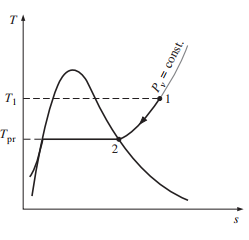
\includegraphics[width=.9\linewidth]{temp_rocio}
	\end{center}
	
	\textbf{Temperatura de bulbo seco $t_{bs}$:} la que medimos en el ambiente con un termómetro ordinario. \\
	
	\textbf{Temperatura de bulbo húmedo $t_{bh}$:} si ahora al bulo del termómetro le colocamos un paño húmedo y le hacemos pasar una corriente de aire, este aire forzará a evaporar el agua del paño por lo que la temperatura del termómetro comenzará a descender. Esto trae como consecuencia un intercambio de calor entre el termómetro y el aire hasta que se estabiliza y la temperatura final del termómetro será la \emph{temperatura de bulbo húmedo}.\\
	
	Siempre $T_{bh} < T_{bs}$. Estas temperaturas serán iguales cando $H_r = 100\%$. Es decir que el aire no tiene mas capacidad de absorber humedad por lo que no va a poder secar el paño.
	
		
	%END_FOLD
	
	
	%TRANSMISION DE CALOR---------------------------------------------------
	%BEGIN_FOLD
		\unidad{16}{Transmición de Calor}
		La ``\textit{transferencia de calor}'' se define como la transmisión de energía de una región a otra como resultado de un gradiente de temperatura, tiene lugar mediante los tres modos siguientes:
	
	\begin{tabular}{l}
		$\bullet$	Conducción\\
		$\bullet$	Convección\\
		$\bullet$	Radiación
	\end{tabular}\\
	
	\textbf{Conducción} es la transferenia de calor de una parte de una sustancia a ora parte de la misma sustancia, o de una sustancia a otra en contacto físico con ella, sin desplazamiento apreciable de las moléculas que forman la sustancia.\\
	\textbf{Convección} es la ransferencia de calor dentro de un fluido al mezclarse una arte del fluido con otra.\\
	\textbf{Radiación} es la transferencia de calor por medios que no sean de conduccióon o convección. Ondas electromagnéticas.\\
	
	\textbf{LEY DE FOURIER DE LA CONDUCCIÓN DE CALOR}\\
	``\textit{La tasa de flujo de calor a través de un sólido simple homogéneo es directamente proporcional al área de la sección transversal del flujo de calor y al cambio de temperatura con respecto a la dirección del flujo de calor}''. Ley basada en evidencia experimental, no derivable del primer principio.\\
	
	\textbf{Conducción de calor a través de paredes planas y compuestas.}
	\begin{center}
		\boxed{Q=\dfrac{A.\Delta T}{\dfrac{1}{h}+\dfrac{L}{k}+\dfrac{1}{h}}}
	\end{center}
	\begin{tabular}{ l} 
		$\bullet Q$ = flujo de calor\\
		$\bullet A$ = área\\
		$\bullet \Delta T$ = cambio de temperatura\\
		$\bullet L$ = longitud de espesor de pared\\
		$\bullet h$ = coef. convección\\
		$\bullet k$ = coef. conducción\\
	\end{tabular}
	
	\textbf{Conducción de calor a través de cilindros huecos y compuestos.}
	\begin{center}
		\boxed{Q=\dfrac{2 \pi.L.\Delta T}{\dfrac{1}{h.r_{i}}+\dfrac{ln\left(\frac{r_{f}}{r_{i}}\right)}{k}+\dfrac{1}{h.r_{f}}}}
	\end{center}
	\begin{tabular}{ l} 
		$\bullet Q$ = flujo de calor\\
		$\bullet r_{i}$ = radio interior de cilindro\\
		$\bullet r_{f}$ = radio exterior de cilindro\\
		$\bullet \Delta T$ = cambio de temperatura\\
		$\bullet L$ = longitud de espesor de pared\\
		$\bullet h$ = coef. convección\\
		$\bullet k$ = coef. conducción\\
	\end{tabular}
	
	%END_FOLD
\end{document}